\chapter{مسیرها و مدارها}

این فصل روی دو نوع مسیر در گراف تمرکز دارد:
\begin{itemize}
\item یک \key{مسیر اویلری} مسیری است که
از هر یال دقیقاً یک بار عبور می‌کند.
\item یک \key{مسیر هامیلتونی} مسیری است
که از هر رأس دقیقاً یک بار بازدید می‌کند.
\end{itemize}

اگرچه مسیرهای اویلری و هامیلتونی در نگاه اول مفاهیم مشابهی به نظر می‌رسند،
مسائل محاسباتی مربوط به آن‌ها بسیار متفاوت است.
مشخص شده قاعده ساده‌ای وجود دارد که تعیین می‌کند آیا یک گراف شامل مسیر اویلری است یا خیر،
و همچنین الگوریتم کارآمدی برای یافتن چنین مسیری در صورت وجود در دست است.
در مقابل، بررسی وجود مسیر هامیلتونی یک مسئله NP-hard است
و هیچ الگوریتم کارآمدی برای حل آن شناخته نشده است.

\section{مسیرهای اویلری}

\index{Eulerian path}

یک \key{مسیر اویلری}\footnote{ل. اویلر چنین مسیرهایی را در سال ۱۷۳۶ هنگامی که مسئله مشهور پل‌های کونیگسبرگ را حل کرد، بررسی نمود. این رویداد نقطه پیدایش نظریه گراف بود.} مسیری است
که دقیقاً یک بار از هر یال گراف عبور می‌کند.
برای مثال، گراف
\begin{center}
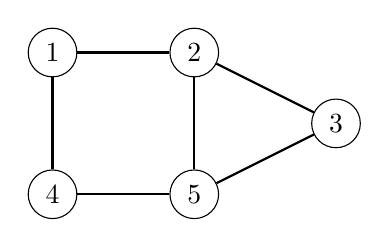
\begin{tikzpicture}[scale=0.9]
\node[draw, circle] (1) at (1,5) {$1$};
\node[draw, circle] (2) at (3,5) {$2$};
\node[draw, circle] (3) at (5,4) {$3$};
\node[draw, circle] (4) at (1,3) {$4$};
\node[draw, circle] (5) at (3,3) {$5$};

\path[draw,thick,-] (1) -- (2);
\path[draw,thick,-] (2) -- (3);
\path[draw,thick,-] (1) -- (4);
\path[draw,thick,-] (3) -- (5);
\path[draw,thick,-] (2) -- (5);
\path[draw,thick,-] (4) -- (5);
\end{tikzpicture}
\end{center}
دارای یک مسیر اویلری از رأس ۲ به رأس ۵ است:
\begin{center}
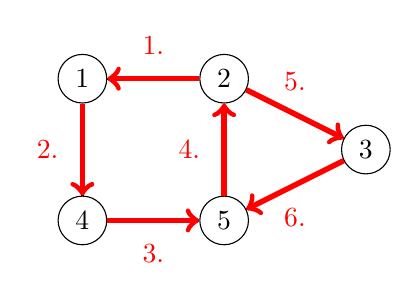
\begin{tikzpicture}[scale=0.9]
\node[draw, circle] (1) at (1,5) {$1$};
\node[draw, circle] (2) at (3,5) {$2$};
\node[draw, circle] (3) at (5,4) {$3$};
\node[draw, circle] (4) at (1,3) {$4$};
\node[draw, circle] (5) at (3,3) {$5$};

\path[draw,thick,-] (1) -- (2);
\path[draw,thick,-] (2) -- (3);
\path[draw,thick,-] (1) -- (4);
\path[draw,thick,-] (3) -- (5);
\path[draw,thick,-] (2) -- (5);
\path[draw,thick,-] (4) -- (5);

\path[draw=red,thick,->,line width=2pt] (2) -- node[font=\small,label={[red]north:1.}] {} (1);
\path[draw=red,thick,->,line width=2pt] (1) -- node[font=\small,label={[red]left:2.}] {} (4);
\path[draw=red,thick,->,line width=2pt] (4) -- node[font=\small,label={[red]south:3.}] {} (5);
\path[draw=red,thick,->,line width=2pt] (5) -- node[font=\small,label={[red]left:4.}] {} (2);
\path[draw=red,thick,->,line width=2pt] (2) -- node[font=\small,label={[red]north:5.}] {} (3);
\path[draw=red,thick,->,line width=2pt] (3) -- node[font=\small,label={[red]south:6.}] {} (5);
\end{tikzpicture}
\end{center}
\index{Eulerian circuit}
یک \key{مدار اویلری}
مسیر اویلری است که در همان رأس شروع، پایان می‌یابد.
برای مثال، گراف
\begin{center}
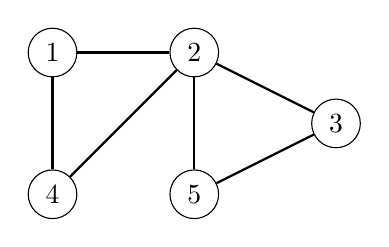
\begin{tikzpicture}[scale=0.9]
\node[draw, circle] (1) at (1,5) {$1$};
\node[draw, circle] (2) at (3,5) {$2$};
\node[draw, circle] (3) at (5,4) {$3$};
\node[draw, circle] (4) at (1,3) {$4$};
\node[draw, circle] (5) at (3,3) {$5$};

\path[draw,thick,-] (1) -- (2);
\path[draw,thick,-] (2) -- (3);
\path[draw,thick,-] (1) -- (4);
\path[draw,thick,-] (3) -- (5);
\path[draw,thick,-] (2) -- (5);
\path[draw,thick,-] (2) -- (4);
\end{tikzpicture}
\end{center}
دارای یک مدار اویلری است که از راس ۱ شروع شده و در راس ۱ پایان می‌یابد:
\begin{center}
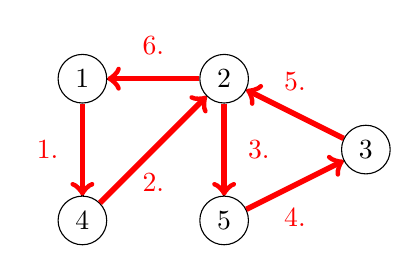
\begin{tikzpicture}[scale=0.9]
\node[draw, circle] (1) at (1,5) {$1$};
\node[draw, circle] (2) at (3,5) {$2$};
\node[draw, circle] (3) at (5,4) {$3$};
\node[draw, circle] (4) at (1,3) {$4$};
\node[draw, circle] (5) at (3,3) {$5$};

\path[draw,thick,-] (1) -- (2);
\path[draw,thick,-] (2) -- (3);
\path[draw,thick,-] (1) -- (4);
\path[draw,thick,-] (3) -- (5);
\path[draw,thick,-] (2) -- (5);
\path[draw,thick,-] (2) -- (4);

\path[draw=red,thick,->,line width=2pt] (1) -- node[font=\small,label={[red]left:1.}] {} (4);
\path[draw=red,thick,->,line width=2pt] (4) -- node[font=\small,label={[red]south:2.}] {} (2);
\path[draw=red,thick,->,line width=2pt] (2) -- node[font=\small,label={[red]right:3.}] {} (5);
\path[draw=red,thick,->,line width=2pt] (5) -- node[font=\small,label={[red]south:4.}] {} (3);
\path[draw=red,thick,->,line width=2pt] (3) -- node[font=\small,label={[red]north:5.}] {} (2);
\path[draw=red,thick,->,line width=2pt] (2) -- node[font=\small,label={[red]north:6.}] {} (1);
\end{tikzpicture}
\end{center}

\subsubsection{شرایط وجود}

وجود مسیرها و مدارهای اویلری
به درجه راس‌ها بستگی دارد.
نخست، یک گراف بدون جهت دارای مسیر اویلری است
دقیقاً زمانی که تمام یال‌ها
به یک مؤلفه همبندی یکسان تعلق داشته باشند و
\begin{itemize}
\item درجه هر راس زوج باشد \emph{یا}
\item درجه دقیقاً دو راس فرد باشد،
و درجه تمام راس‌های دیگر زوج باشد.
\end{itemize}

در حالت اول، هر مسیر اویلری یک مدار اویلری نیز هست.
در حالت دوم، راس‌های با درجه فرد، راس‌های شروع
و پایان یک مسیر اویلری هستند که مدار اویلری نیست.

\begin{samepage}
به عنوان مثال، در گراف
\begin{center}
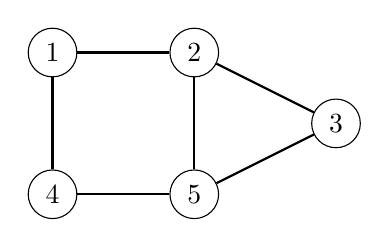
\begin{tikzpicture}[scale=0.9]
\node[draw, circle] (1) at (1,5) {$1$};
\node[draw, circle] (2) at (3,5) {$2$};
\node[draw, circle] (3) at (5,4) {$3$};
\node[draw, circle] (4) at (1,3) {$4$};
\node[draw, circle] (5) at (3,3) {$5$};

\path[draw,thick,-] (1) -- (2);
\path[draw,thick,-] (2) -- (3);
\path[draw,thick,-] (1) -- (4);
\path[draw,thick,-] (3) -- (5);
\path[draw,thick,-] (2) -- (5);
\path[draw,thick,-] (4) -- (5);
\end{tikzpicture}
\end{center}
\end{samepage}
راس‌های ۱، ۳ و ۴ دارای درجه ۲ هستند،
و راس‌های ۲ و ۵ دارای درجه ۳ هستند.
دقیقاً دو راس درجه فرد دارند،
بنابراین یک مسیر اویلری بین راس‌های ۲ و ۵ وجود دارد،
اما گراف شامل هیچ مدار اویلری نیست.

در گراف جهت‌دار،
تمرکز روی درجه‌های ورودی و خروجی
راس‌ها است.
گراف جهت‌دار دقیقا زمانی شامل مسیر اویلری است
که همه یال‌ها متعلق به یک مولفه همبند
باشند و
\begin{itemize}
\item در هر راس، درجه ورودی برابر با درجه خروجی باشد، \emph{یا}
\item در یک راس، درجه ورودی یکی بیشتر از درجه خروجی باشد،
در راسی دیگر، درجه خروجی یکی بیشتر از درجه ورودی باشد،
و در تمام راس‌های دیگر، درجه ورودی برابر با درجه خروجی باشد.
\end{itemize}

در حالت اول، هر مسیر اویلری
یک دور اویلری نیز هست،
و در حالت دوم، گراف شامل مسیر اویلری است
که از راسی با درجه خروجی بزرگ‌تر شروع می‌شود
و در راسی با درجه ورودی بزرگ‌تر پایان می‌یابد.

برای مثال، در گراف
\begin{center}
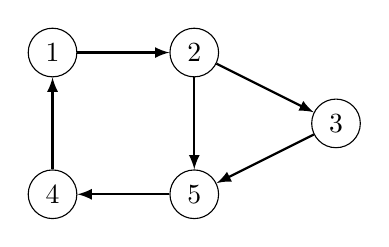
\begin{tikzpicture}[scale=0.9]
\node[draw, circle] (1) at (1,5) {$1$};
\node[draw, circle] (2) at (3,5) {$2$};
\node[draw, circle] (3) at (5,4) {$3$};
\node[draw, circle] (4) at (1,3) {$4$};
\node[draw, circle] (5) at (3,3) {$5$};

\path[draw,thick,->,>=latex] (1) -- (2);
\path[draw,thick,->,>=latex] (2) -- (3);
\path[draw,thick,->,>=latex] (4) -- (1);
\path[draw,thick,->,>=latex] (3) -- (5);
\path[draw,thick,->,>=latex] (2) -- (5);
\path[draw,thick,->,>=latex] (5) -- (4);
\end{tikzpicture}
\end{center}
راس‌های ۱، ۳ و ۴ همگی دارای درجه ورودی ۱ و درجه خروجی ۱ هستند،
راس ۲ دارای درجه ورودی ۱ و درجه خروجی ۲ است،
و راس ۵ دارای درجه ورودی ۲ و درجه خروجی ۱ است.
بنابراین، گراف شامل یک مسیر اویلری
از راس ۲ به راس ۵ است:
\begin{center}
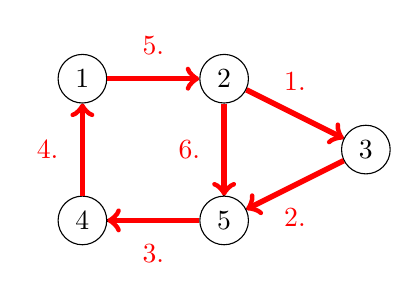
\begin{tikzpicture}[scale=0.9]
\node[draw, circle] (1) at (1,5) {$1$};
\node[draw, circle] (2) at (3,5) {$2$};
\node[draw, circle] (3) at (5,4) {$3$};
\node[draw, circle] (4) at (1,3) {$4$};
\node[draw, circle] (5) at (3,3) {$5$};

\path[draw,thick,-] (1) -- (2);
\path[draw,thick,-] (2) -- (3);
\path[draw,thick,-] (1) -- (4);
\path[draw,thick,-] (3) -- (5);
\path[draw,thick,-] (2) -- (5);
\path[draw,thick,-] (4) -- (5);

\path[draw=red,thick,->,line width=2pt] (2) -- node[font=\small,label={[red]north:1.}] {} (3);
\path[draw=red,thick,->,line width=2pt] (3) -- node[font=\small,label={[red]south:2.}] {} (5);
\path[draw=red,thick,->,line width=2pt] (5) -- node[font=\small,label={[red]south:3.}] {} (4);
\path[draw=red,thick,->,line width=2pt] (4) -- node[font=\small,label={[red]left:4.}] {} (1);
\path[draw=red,thick,->,line width=2pt] (1) -- node[font=\small,label={[red]north:5.}] {} (2);
\path[draw=red,thick,->,line width=2pt] (2) -- node[font=\small,label={[red]left:6.}] {} (5);
\end{tikzpicture}
\end{center}

\subsubsection{الگوریتم هیرهولتزر}

\index{Hierholzer's algorithm}

\key{الگوریتم هیرهولتزر}\footnote{این الگوریتم در سال ۱۸۷۳ پس از مرگ هیرهولتزر منتشر شد \cite{hie73}.} روشی کارآمد
برای ساخت
دور اویلری است.
الگوریتم از چند مرحله تشکیل شده است
که هر مرحله یال‌های جدیدی به دور اضافه می‌کند.
البته فرض بر این است که گراف شامل
دور اویلری باشد؛ در غیر این صورت الگوریتم هیرهولتزر
نمی‌تواند آن را پیدا کند.

ابتدا، الگوریتم مداری می‌سازد که شامل
برخی از یال‌های گراف است (نه لزوماً همه آن‌ها).
سپس الگوریتم مدار را گام‌به‌گام با افزودن زیرمدارها
گسترش می‌دهد.
این فرایند تا افزوده‌شدن تمام یال‌ها
به مدار ادامه می‌یابد.

الگوریتم با یافتن گره $x$ که متعلق به مدار است
ولی یال خروجی خارج از مدار دارد، مدار را گسترش می‌دهد.
الگوریتم مسیر جدیدی از گره $x$ می‌سازد
که فقط شامل یال‌های خارج از مدار است.
در نهایت، مسیر به گره $x$ بازمی‌گردد
و یک زیرمدار ایجاد می‌کند.

اگر گراف فقط شامل مسیر اویلری باشد،
همچنان می‌توان از الگوریتم هیرهولتزر استفاده کرد؛
کافی است یال اضافی به گراف اضافه شود
و پس از ساخت مدار، آن یال حذف گردد.
مثلاً در گراف غیرجهت‌دار،
یال اضافی بین دو گره با درجه فرد اضافه می‌شود.

در ادامه، نحوه ساخت مدار اویلری در گراف غیرجهت‌دار
با الگوریتم هیرهولتزر نشان داده می‌شود.

\subsubsection{مثال}

\begin{samepage}
گراف زیر را در نظر بگیرید:
\begin{center}
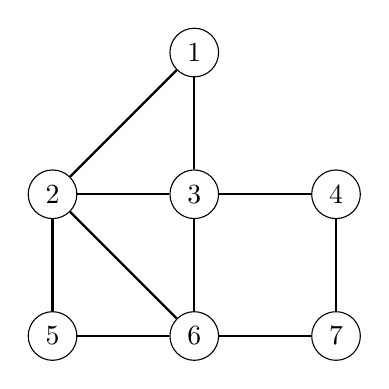
\begin{tikzpicture}[scale=0.9]
\node[draw, circle] (1) at (3,5) {$1$};
\node[draw, circle] (2) at (1,3) {$2$};
\node[draw, circle] (3) at (3,3) {$3$};
\node[draw, circle] (4) at (5,3) {$4$};
\node[draw, circle] (5) at (1,1) {$5$};
\node[draw, circle] (6) at (3,1) {$6$};
\node[draw, circle] (7) at (5,1) {$7$};

\path[draw,thick,-] (1) -- (2);
\path[draw,thick,-] (1) -- (3);
\path[draw,thick,-] (2) -- (3);
\path[draw,thick,-] (2) -- (5);
\path[draw,thick,-] (2) -- (6);
\path[draw,thick,-] (3) -- (4);
\path[draw,thick,-] (3) -- (6);
\path[draw,thick,-] (4) -- (7);
\path[draw,thick,-] (5) -- (6);
\path[draw,thick,-] (6) -- (7);
\end{tikzpicture}
\end{center}
\end{samepage}

\begin{samepage}
فرض کنید الگوریتم ابتدا مداری از گره ۱ بسازد.
یک مدار ممکن
$1 \rightarrow 2 \rightarrow 3 \rightarrow 1$ است:
\begin{center}
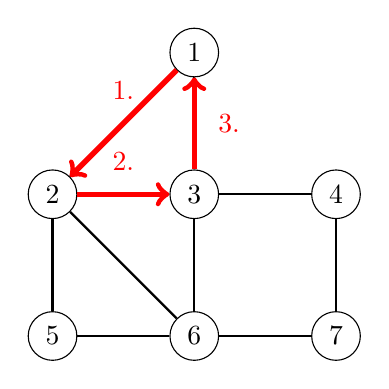
\begin{tikzpicture}[scale=0.9]
\node[draw, circle] (1) at (3,5) {$1$};
\node[draw, circle] (2) at (1,3) {$2$};
\node[draw, circle] (3) at (3,3) {$3$};
\node[draw, circle] (4) at (5,3) {$4$};
\node[draw, circle] (5) at (1,1) {$5$};
\node[draw, circle] (6) at (3,1) {$6$};
\node[draw, circle] (7) at (5,1) {$7$};

\path[draw,thick,-] (1) -- (2);
\path[draw,thick,-] (1) -- (3);
\path[draw,thick,-] (2) -- (3);
\path[draw,thick,-] (2) -- (5);
\path[draw,thick,-] (2) -- (6);
\path[draw,thick,-] (3) -- (4);
\path[draw,thick,-] (3) -- (6);
\path[draw,thick,-] (4) -- (7);
\path[draw,thick,-] (5) -- (6);
\path[draw,thick,-] (6) -- (7);

\path[draw=red,thick,->,line width=2pt] (1) -- node[font=\small,label={[red]north:1.}] {} (2);
\path[draw=red,thick,->,line width=2pt] (2) -- node[font=\small,label={[red]north:2.}] {} (3);
\path[draw=red,thick,->,line width=2pt] (3) -- node[font=\small,label={[red]east:3.}] {} (1);
\end{tikzpicture}
\end{center}
\end{samepage}
پس از این، الگوریتم زیرمدار
$2 \rightarrow 5 \rightarrow 6 \rightarrow 2$
را به مدار اضافه می‌کند:
\begin{center}
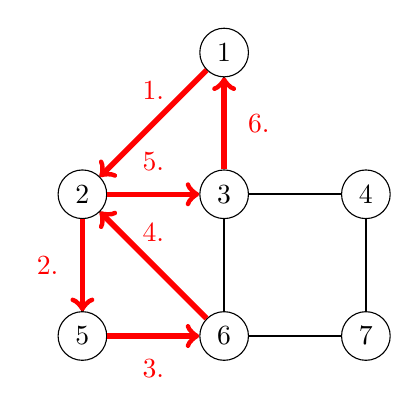
\begin{tikzpicture}[scale=0.9]
\node[draw, circle] (1) at (3,5) {$1$};
\node[draw, circle] (2) at (1,3) {$2$};
\node[draw, circle] (3) at (3,3) {$3$};
\node[draw, circle] (4) at (5,3) {$4$};
\node[draw, circle] (5) at (1,1) {$5$};
\node[draw, circle] (6) at (3,1) {$6$};
\node[draw, circle] (7) at (5,1) {$7$};

\path[draw,thick,-] (1) -- (2);
\path[draw,thick,-] (1) -- (3);
\path[draw,thick,-] (2) -- (3);
\path[draw,thick,-] (2) -- (5);
\path[draw,thick,-] (2) -- (6);
\path[draw,thick,-] (3) -- (4);
\path[draw,thick,-] (3) -- (6);
\path[draw,thick,-] (4) -- (7);
\path[draw,thick,-] (5) -- (6);
\path[draw,thick,-] (6) -- (7);

\path[draw=red,thick,->,line width=2pt] (1) -- node[font=\small,label={[red]north:1.}] {} (2);
\path[draw=red,thick,->,line width=2pt] (2) -- node[font=\small,label={[red]west:2.}] {} (5);
\path[draw=red,thick,->,line width=2pt] (5) -- node[font=\small,label={[red]south:3.}] {} (6);
\path[draw=red,thick,->,line width=2pt] (6) -- node[font=\small,label={[red]north:4.}] {} (2);
\path[draw=red,thick,->,line width=2pt] (2) -- node[font=\small,label={[red]north:5.}] {} (3);
\path[draw=red,thick,->,line width=2pt] (3) -- node[font=\small,label={[red]east:6.}] {} (1);
\end{tikzpicture}
\end{center}
در نهایت، الگوریتم زیرمدار
$6 \rightarrow 3 \rightarrow 4 \rightarrow 7 \rightarrow 6$
را به مدار اضافه می‌کند:
\begin{center}
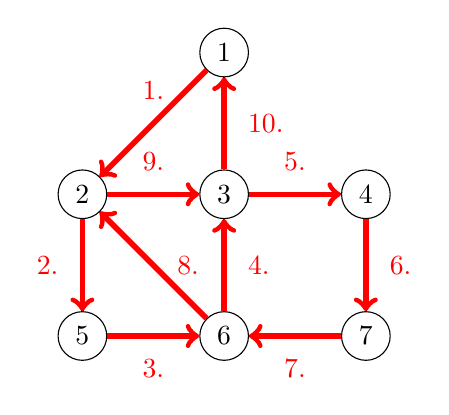
\begin{tikzpicture}[scale=0.9]
\node[draw, circle] (1) at (3,5) {$1$};
\node[draw, circle] (2) at (1,3) {$2$};
\node[draw, circle] (3) at (3,3) {$3$};
\node[draw, circle] (4) at (5,3) {$4$};
\node[draw, circle] (5) at (1,1) {$5$};
\node[draw, circle] (6) at (3,1) {$6$};
\node[draw, circle] (7) at (5,1) {$7$};

\path[draw,thick,-] (1) -- (2);
\path[draw,thick,-] (1) -- (3);
\path[draw,thick,-] (2) -- (3);
\path[draw,thick,-] (2) -- (5);
\path[draw,thick,-] (2) -- (6);
\path[draw,thick,-] (3) -- (4);
\path[draw,thick,-] (3) -- (6);
\path[draw,thick,-] (4) -- (7);
\path[draw,thick,-] (5) -- (6);
\path[draw,thick,-] (6) -- (7);

\path[draw=red,thick,->,line width=2pt] (1) -- node[font=\small,label={[red]north:1.}] {} (2);
\path[draw=red,thick,->,line width=2pt] (2) -- node[font=\small,label={[red]west:2.}] {} (5);
\path[draw=red,thick,->,line width=2pt] (5) -- node[font=\small,label={[red]south:3.}] {} (6);
\path[draw=red,thick,->,line width=2pt] (6) -- node[font=\small,label={[red]east:4.}] {} (3);
\path[draw=red,thick,->,line width=2pt] (3) -- node[font=\small,label={[red]north:5.}] {} (4);
\path[draw=red,thick,->,line width=2pt] (4) -- node[font=\small,label={[red]east:6.}] {} (7);
\path[draw=red,thick,->,line width=2pt] (7) -- node[font=\small,label={[red]south:7.}] {} (6);
\path[draw=red,thick,->,line width=2pt] (6) -- node[font=\small,label={[red]right:8.}] {} (2);
\path[draw=red,thick,->,line width=2pt] (2) -- node[font=\small,label={[red]north:9.}] {} (3);
\path[draw=red,thick,->,line width=2pt] (3) -- node[font=\small,label={[red]east:10.}] {} (1);
\end{tikzpicture}
\end{center}
اکنون تمام یال‌ها در مدار گنجانده شده‌اند،
بنابراین یک مدار اویلری با موفقیت ساخته شد.

\section{مسیرهای همیلتونی}

\index{Hamiltonian path@مسیر همیلتونی}

یک \key{مسیر همیلتونی}
%\footnote{W. R. Hamilton (1805--1865) was an Irish mathematician.}
مسیری است
که دقیقاً یک بار از هر رأس گراف عبور می‌کند.
به عنوان مثال، گراف
\begin{center}
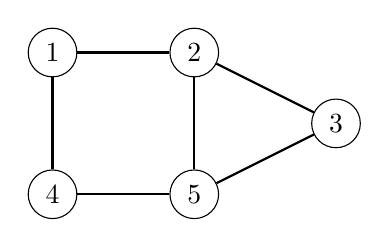
\begin{tikzpicture}[scale=0.9]
\node[draw, circle] (1) at (1,5) {$1$};
\node[draw, circle] (2) at (3,5) {$2$};
\node[draw, circle] (3) at (5,4) {$3$};
\node[draw, circle] (4) at (1,3) {$4$};
\node[draw, circle] (5) at (3,3) {$5$};

\path[draw,thick,-] (1) -- (2);
\path[draw,thick,-] (2) -- (3);
\path[draw,thick,-] (1) -- (4);
\path[draw,thick,-] (3) -- (5);
\path[draw,thick,-] (2) -- (5);
\path[draw,thick,-] (4) -- (5);
\end{tikzpicture}
\end{center}
شامل یک مسیر همیلتونی از رأس 1 به رأس 3 است:
\begin{center}
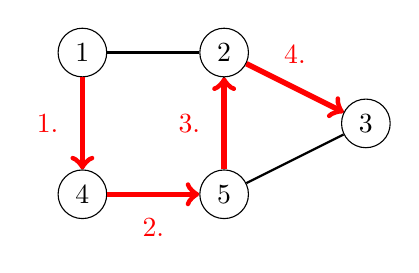
\begin{tikzpicture}[scale=0.9]
\node[draw, circle] (1) at (1,5) {$1$};
\node[draw, circle] (2) at (3,5) {$2$};
\node[draw, circle] (3) at (5,4) {$3$};
\node[draw, circle] (4) at (1,3) {$4$};
\node[draw, circle] (5) at (3,3) {$5$};

\path[draw,thick,-] (1) -- (2);
\path[draw,thick,-] (2) -- (3);
\path[draw,thick,-] (1) -- (4);
\path[draw,thick,-] (3) -- (5);
\path[draw,thick,-] (2) -- (5);
\path[draw,thick,-] (4) -- (5);

\path[draw=red,thick,->,line width=2pt] (1) -- node[font=\small,label={[red]left:1.}] {} (4);
\path[draw=red,thick,->,line width=2pt] (4) -- node[font=\small,label={[red]south:2.}] {} (5);
\path[draw=red,thick,->,line width=2pt] (5) -- node[font=\small,label={[red]left:3.}] {} (2);
\path[draw=red,thick,->,line width=2pt] (2) -- node[font=\small,label={[red]north:4.}] {} (3);
\end{tikzpicture}
\end{center}

\index{Hamiltonian circuit@مدار همیلتونی}

اگر یک مسیر هامیلتونی در همان رأس شروع، پایان یابد،
\key{دور هامیلتونی} نامیده می‌شود.
گراف بالا دارای یک دور هامیلتونی نیز هست
که از رأس ۱ شروع و به آن ختم می‌شود:
\begin{center}
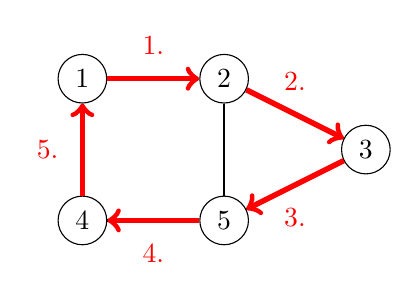
\begin{tikzpicture}[scale=0.9]
\node[draw, circle] (1) at (1,5) {$1$};
\node[draw, circle] (2) at (3,5) {$2$};
\node[draw, circle] (3) at (5,4) {$3$};
\node[draw, circle] (4) at (1,3) {$4$};
\node[draw, circle] (5) at (3,3) {$5$};

\path[draw,thick,-] (1) -- (2);
\path[draw,thick,-] (2) -- (3);
\path[draw,thick,-] (1) -- (4);
\path[draw,thick,-] (3) -- (5);
\path[draw,thick,-] (2) -- (5);
\path[draw,thick,-] (4) -- (5);

\path[draw=red,thick,->,line width=2pt] (1) -- node[font=\small,label={[red]north:1.}] {} (2);
\path[draw=red,thick,->,line width=2pt] (2) -- node[font=\small,label={[red]north:2.}] {} (3);
\path[draw=red,thick,->,line width=2pt] (3) -- node[font=\small,label={[red]south:3.}] {} (5);
\path[draw=red,thick,->,line width=2pt] (5) -- node[font=\small,label={[red]south:4.}] {} (4);
\path[draw=red,thick,->,line width=2pt] (4) -- node[font=\small,label={[red]left:5.}] {} (1);
\end{tikzpicture}
\end{center}

\subsubsection{وجود}

هیچ روش کارآمدی برای بررسی وجود مسیر هامیلتونی در یک گراف
شناخته نشده است و این مسئله NP-hard است.
با این حال، در برخی حالت‌های خاص می‌توان مطمئن بود
که گراف حاوی مسیر هامیلتونی است.

یک مشاهده ساده این است که اگر گراف کامل باشد،
یعنی بین هر جفت رأس یک یال وجود داشته باشد،
حاوی مسیر هامیلتونی نیز هست.
همچنین نتایج قوی‌تری به دست آمده است:

\begin{itemize}
\item
\index{Dirac's theorem}
\key{قضیه دیراک}: %\cite{dir52}
اگر درجه هر رأس حداقل $n/2$ باشد،
گراف شامل مسیر هامیلتونی است.
\item
\index{Ore's theorem}
\key{قضیه اور}: %\cite{ore60}
اگر مجموع درجات هر جفت رأس غیرمجاور
حداقل $n$ باشد،
گراف شامل مسیر هامیلتونی است.
\end{itemize}

ویژگی مشترک این قضایا و نتایج دیگر این است
که اگر گراف دارای \emph{تعداد زیادی} یال باشد،
وجود مسیر هامیلتونی را تضمین می‌کنند.
این امر منطقی است، زیرا هرچه گراف یال‌های بیشتری داشته باشد،
امکان‌های بیشتری برای ساخت یک مسیر هامیلتونی وجود دارد.

\subsubsection{ساخت}

از آنجا که روش کارآمدی برای بررسی وجود مسیر هامیلتونی
وجود ندارد، مشخص است که روشی نیز برای ساخت کارآمد
این مسیر وجود ندارد، زیرا در غیر این صورت
می‌توانستیم تلاش کنیم مسیر را بسازیم و ببینیم
آیا وجود دارد یا خیر.

یک روش ساده برای جستجوی مسیر هامیلتونی
استفاده از الگوریتم عقب‌گرد است که تمام
حالت‌های ممکن برای ساخت مسیر را بررسی می‌کند.
پیچیدگی زمانی چنین الگوریتمی حداقل $O(n!)$ است،
زیرا $n!$ روش مختلف برای انتخاب ترتیب $n$ رأس وجود دارد.

یک راهکار کارآمدتر مبتنی بر برنامه‌نویسی پویا است
(فصل ۱۰.۵ را ببینید).
ایده محاسبه مقادیر
تابع $\texttt{possible}(S,x)$ است،
که در آن $S$ زیرمجموعه‌ای از رأس‌ها و $x$
یکی از رأس‌ها است.
تابع مشخص می‌کند آیا مسیر همیلتونی وجود دارد
که رأس‌های $S$ را پیمایش کند و در رأس $x$ پایان یابد.
پیاده‌سازی این راهکار در زمان $O(2^n n^2)$ ممکن است.

\section{دنباله‌های دی بروین}

\index{دنباله دی بروین}

یک \key{دنباله دی بروین}
رشته‌ای است که شامل
هر رشته به طول $n$
دقیقاً یک بار به عنوان زیررشته است، برای یک
الفبای ثابت با $k$ نویسه.
طول چنین رشته‌ای
$k^n+n-1$ نویسه است.
به عنوان مثال، وقتی $n=3$ و $k=2$ باشد،
یک نمونه از دنباله دی بروین برابر است با
\[0001011100.\]
زیررشته‌های این رشته تمام
ترکیبات سه بیتی هستند:
000، 001، 010، 011، 100، 101، 110 و 111.

مشخص می‌شود هر دنباله دی بروین
متناظر با یک مسیر اویلری در یک گراف است.
ایده ساخت گرافی است که در آن
هر رأس شامل یک رشته از $n-1$ نویسه باشد
و هر یال یک نویسه به رشته اضافه کند.
گراف زیر متناظر با سناریوی بالاست:

\begin{center}
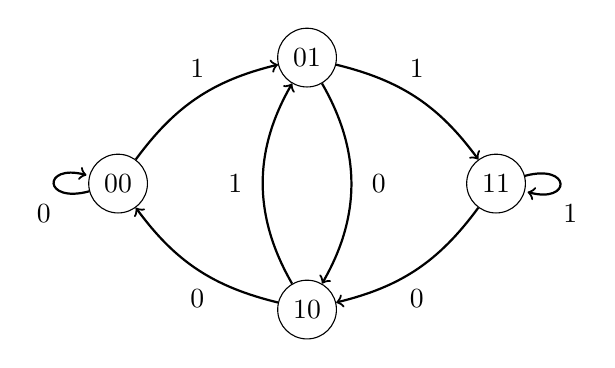
\begin{tikzpicture}[scale=0.8]
\node[draw, circle] (00) at (-3,0) {00};
\node[draw, circle] (11) at (3,0) {11};
\node[draw, circle] (01) at (0,2) {01};
\node[draw, circle] (10) at (0,-2) {10};

\path[draw,thick,->] (00) edge [bend left=20] node[font=\small,label=1] {} (01);
\path[draw,thick,->] (01) edge [bend left=20] node[font=\small,label=1] {} (11);
\path[draw,thick,->] (11) edge [bend left=20] node[font=\small,label=below:0] {} (10);
\path[draw,thick,->] (10) edge [bend left=20] node[font=\small,label=below:0] {} (00);

\path[draw,thick,->] (01) edge [bend left=30] node[font=\small,label=right:0] {} (10);
\path[draw,thick,->] (10) edge [bend left=30] node[font=\small,label=left:1] {} (01);

\path[draw,thick,-] (00) edge [loop left] node[font=\small,label=below:0] {} (00);
\path[draw,thick,-] (11) edge [loop right] node[font=\small,label=below:1] {} (11);
\end{tikzpicture}
\end{center}

یک مسیر اویلری در این گراف متناظر با رشته‌ای است
که شامل تمام رشته‌های به طول $n$ باشد.
رشته شامل نویسه‌های رأس شروع
و تمام نویسه‌های یال‌ها است.
رأس شروع دارای $n-1$ نویسه است
و $k^n$ نویسه در یال‌ها وجود دارد،
بنابراین طول رشته $k^n+n-1$ است.

\section{گشت‌های اسب}

\index{گشت اسب}

یک \key{گشت اسب} دنباله‌ای از حرکات
یک اسب روی صفحه شطرنج $n \times n$
طبق قوانین شطرنج است به طوری که اسب
هر خانه را دقیقاً یک بار ملاقات کند.
یک گشت اسب \emph{بسته} نامیده می‌شود
اگر اسب در نهایت به خانه شروع برگردد و
در غیر این صورت یک گشت \emph{باز} نامیده می‌شود.

به عنوان مثال، در اینجا یک گشت اسب باز روی صفحه $5 \times 5$ آمده است:

\begin{center}
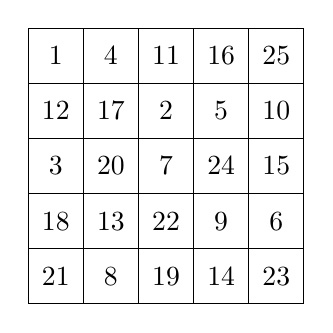
\begin{tikzpicture}[scale=0.7]
\draw (0,0) grid (5,5);
\node at (0.5,4.5) {$1$};
\node at (1.5,4.5) {$4$};
\node at (2.5,4.5) {$11$};
\node at (3.5,4.5) {$16$};
\node at (4.5,4.5) {$25$};
\node at (0.5,3.5) {$12$};
\node at (1.5,3.5) {$17$};
\node at (2.5,3.5) {$2$};
\node at (3.5,3.5) {$5$};
\node at (4.5,3.5) {$10$};
\node at (0.5,2.5) {$3$};
\node at (1.5,2.5) {$20$};
\node at (2.5,2.5) {$7$};
\node at (3.5,2.5) {$24$};
\node at (4.5,2.5) {$15$};
\node at (0.5,1.5) {$18$};
\node at (1.5,1.5) {$13$};
\node at (2.5,1.5) {$22$};
\node at (3.5,1.5) {$9$};
\node at (4.5,1.5) {$6$};
\node at (0.5,0.5) {$21$};
\node at (1.5,0.5) {$8$};
\node at (2.5,0.5) {$19$};
\node at (3.5,0.5) {$14$};
\node at (4.5,0.5) {$23$};
\end{tikzpicture}
\end{center}

گشت اسب معادل مسیر همیلتونی در گرافی است
که رأس‌های آن خانه‌های صفحه شطرنج هستند،
و دو رأس با یال به هم متصل‌اند اگر اسب
طبق قوانین شطرنج بتواند بین آن خانه‌ها حرکت کند.

یک روش طبیعی برای ساخت گشت اسب، روش عقب‌گرد است.
می‌توان با استفاده از \emph{روش‌های ابتکاری} (heuristics) که اسب را
برای یافتن سریع گشت کامل هدایت می‌کنند،
کارایی جستجو را افزایش داد.

\subsubsection{قاعده وارنسدورف}

\index{روش ابتکاری}
\index{قاعده وارنسدورف}

\key{قاعده وارنسدورف} روشی ابتکاری، ساده و کارآمد
برای یافتن گشت اسب است\footnote{این روش ابتکاری در
کتاب وارنسدورف \cite{war23} در سال ۱۸۲۳ پیشنهاد شد. همچنین الگوریتم‌های چندجمله‌ای
برای یافتن گشت اسب وجود دارند \cite{par97}، اما پیچیده‌ترند.}.
با استفاده از این قاعده، ساخت کارآمد گشت حتی
در صفحه‌های بزرگ نیز ممکن است.
ایده این است: اسب همواره به خانه‌ای برود
که تعداد حرکات ممکن بعدی از آن خانه تا حد امکان \emph{کمترین} باشد.

برای مثال، در وضعیت زیر، پنج خانه ممکن وجود دارد
که اسب می‌تواند به آن‌ها برود (خانه‌های $a \ldots e$):
\begin{center}
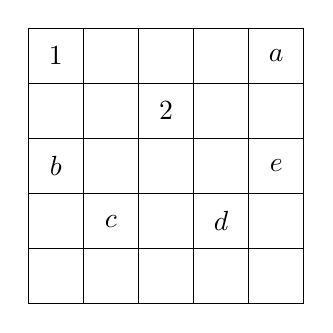
\begin{tikzpicture}[scale=0.7]
\draw (0,0) grid (5,5);
\node at (0.5,4.5) {$1$};
\node at (2.5,3.5) {$2$};
\node at (4.5,4.5) {$a$};
\node at (0.5,2.5) {$b$};
\node at (4.5,2.5) {$e$};
\node at (1.5,1.5) {$c$};
\node at (3.5,1.5) {$d$};
\end{tikzpicture}
\end{center}
در این وضعیت، قاعده وارنسدورف اسب را به خانه $a$ می‌برد،
زیرا پس از این انتخاب، تنها یک حرکت ممکن باقی می‌ماند.
انتخاب‌های دیگر اسب را به خانه‌هایی می‌برند
که از آن‌ها سه حرکت ممکن وجود دارد.